\documentclass{beamer}
\usetheme{Montpellier}
\usecolortheme{beaver}

\title{Rust Remote.Access.Trojan}
\author{Antoine MARTIN, Wesley EDE\\Amad MOHAMMAD, Denis REMACLE}

\begin{document}

  \begin{frame}
 \maketitle
  \end{frame}

\begin{frame}{Sommaire}
    \tableofcontents
\end{frame}

\section{Qu'est-ce qu'un Remote.Access.Trojan ?}
  \begin{frame}{Qu'est-ce qu'un Remote.Access.Trojan ?}
  \begin{itemize}
	\item Un R.A.T est un logiciel qui n'est pas forcément malveillant et qui permet la prise de contrôle à distance d'un PC
	\item Dans nôtre cas c'est un malware qui permet de prendre controle à distance et exécuter des commandes sur un poste ou un ensemble de postes infecté(s).
	\newline
	\item Exemples notables : DarkComet, NanoCore, NJRat...
  \end{itemize}
  \end{frame}

\section{Pourquoi un R.A.T ?}
  \begin{frame}{Pourquoi un R.A.T ?}
  \begin{itemize}
	\item Un challenge stimulant et enrichissant
	\item Choix cohérent avec les compétences diverses du groupe
	\item Une occasion d'apprendre un langage dont l'importance ne fait que croitre
  \end{itemize}
  \end{frame}



\section{Mais pourquoi en RUST absolument ?}
  \begin{frame}{Mais pourquoi en RUST absolument ?}
  \begin{itemize}
	\item Un langage permettant un code "sur" orienté bas niveau
	\item Un langage qui prends sans cesse de l'importance de part son utilisation : noyau linux, moteur HTML de firefox, etc.
	\item Une communaute grandissante et active
  \end{itemize}
  \end{frame}


\section{Comment fonctionne-t-il en somme ?}
  \begin{frame}{Comment fonctionne-t-il en somme ?}
  \begin{itemize}
	\item Kptain-Ratz est capable pour l'instant :
	\item D'utiliser le port 53 en UDP pour se camoufler parmis les flux DNS
	\item D'envoyer un heartbeat a intervalle aléatoire allant de 30 min à 1 heure, le serveur est capable de l'interpréter et d'envoyer les insctructions dans la réponse au heartbeat
	\item Il est codé en RUST
  \end{itemize}
  \end{frame}


\section{Etat des avancements}
  \begin{frame}{Etat des avancements}
  \begin{itemize}
	\item Mise en revue du GAANT associé au Projet 
	\item Différentes difficultées rencontrées
  \end{itemize}
  \end{frame}

\section{}
  \begin{frame}{}
  \begin{itemize}
	\item 
	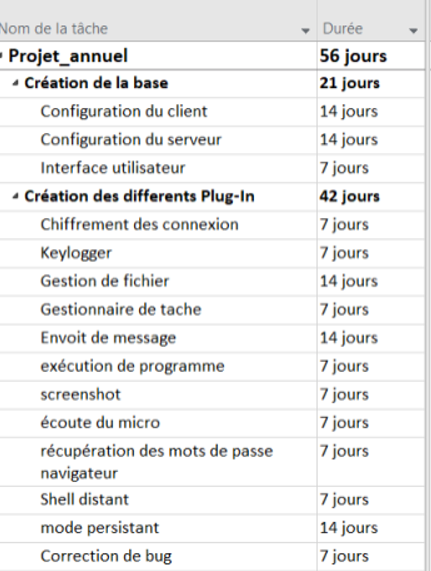
\includegraphics[scale=.5]{gaant1.png}
  \end{itemize}
  \end{frame}

\section{}
  \begin{frame}{}
  \begin{itemize}
	\item 
	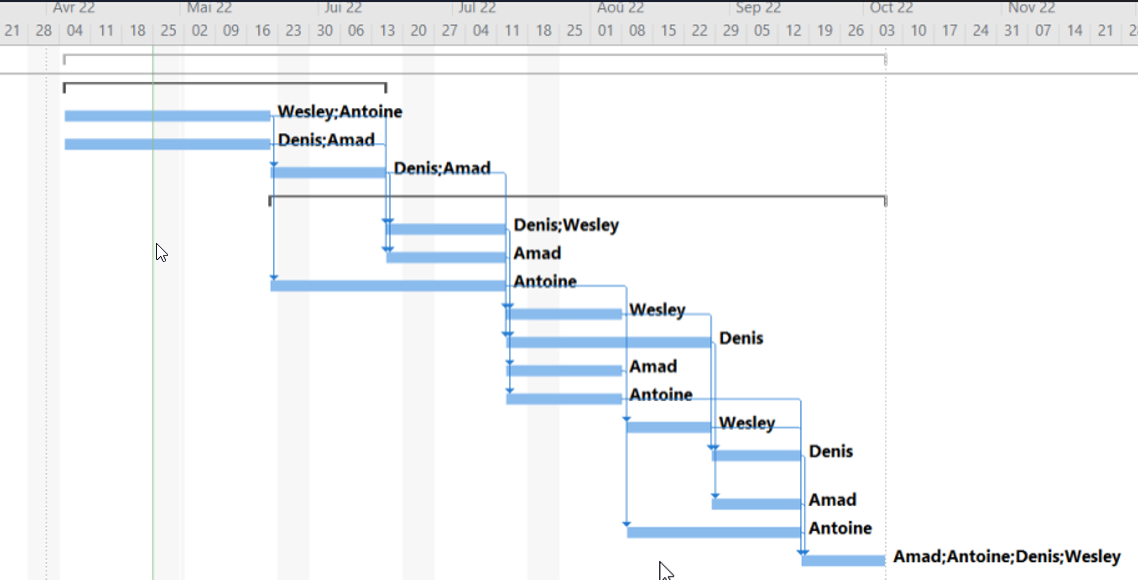
\includegraphics[scale=.4]{gaant2.png}
  \end{itemize}
  \end{frame}

% POC 
\section{PoC de notre solution}
  \begin{frame}{PoC de notre solution}
  \begin{itemize}
	\item Voici les étapes qui constituent l'initiation d'une connexion entre le client et le serveur :
	\item Chiffrement de la connexion
	\item Envoi des instructions
	\item Réception et interprétation du Heartbeat envoyé par le client 
  \end{itemize}
  \end{frame}

\section{PoC de notre solution (Démonstration)}
  \begin{frame}{PoC de notre solution (Démonstration)}
  \begin{itemize}
	\item 
	 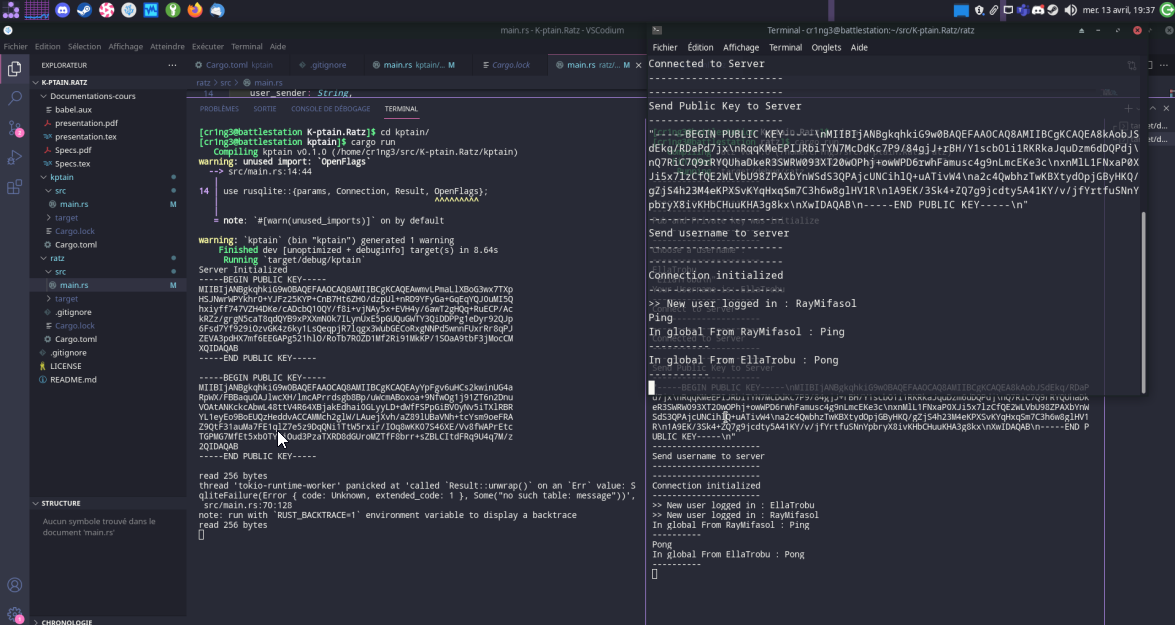
\includegraphics[scale=.4]{poc.png}
  \end{itemize}
  \end{frame}

\section{Batterie de fonctionnalités restant à implémenter}
  \begin{frame}{Batterie de fonctionnalités restant à implémenter}
  \begin{itemize}
	\item Une interface graphique, des fonctionnalités diverses :
	\item Keylogger, Remote Desktop, SCP etc.
	\item L'interface cible devra être semblable à celle-ci :
  \end{itemize}
  \end{frame}

\section{}
  \begin{frame}{}
  \begin{itemize}
	\item
	 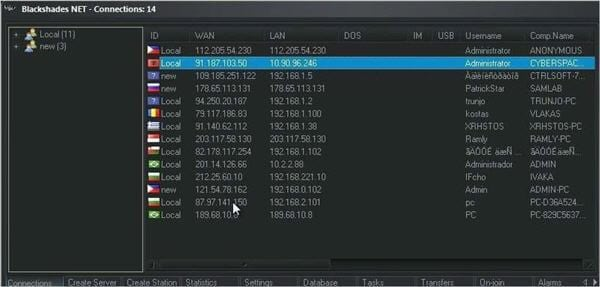
\includegraphics[scale=.5]{blackshades.jpeg}
  \end{itemize}
  \end{frame}



\end{document}
